\documentclass{article}
\usepackage[utf8]{inputenc}
\usepackage{amsmath}
\usepackage{mathenv}
\usepackage{color}
\usepackage{hyperref}
\usepackage{listings}
\usepackage{graphicx}
\usepackage{amssymb}
\usepackage{color} 
\usepackage{hyperref}
\usepackage{array}
\usepackage{placeins}
\usepackage{listings}
\usepackage{fancyhdr}
\usepackage[left=1cm,right=1cm,top=1cm,bottom=1.3cm]{geometry}
\usepackage{accents}


%%%%%%%%%%%%%%%%%%%%%%-----------------------------------------%%%%%%%%%%%%%%%%%%%%%%
% Definition to put a bar under a letter/word (to use with matrix)
\newcommand{\ubar}[1]{\underaccent{\bar}{#1}}

%%%%%%%%%%%%%%%%%%%%%%-----------------------------------------%%%%%%%%%%%%%%%%%%%%%%
% Definition of a column vector
\newcount\colveccount
\newcommand*\colvec[1]{
        \global\colveccount#1
        \begin{pmatrix}
        \colvecnext
}
\def\colvecnext#1{
        #1
        \global\advance\colveccount-1
        \ifnum\colveccount>0
                \\
                \expandafter\colvecnext
        \else
                \end{pmatrix}
        \fi
}

%%%%%%%%%%%%%%%%%%%%%%-----------------------------------------%%%%%%%%%%%%%%%%%%%%%%
% Setting of the logo every page except the first
\fancyhf{}% Clear all headers/footers
\fancyfoot[L]{
\includegraphics[height=1.3cm]{epl-logo.jpg}} 
\pagestyle{fancy} 
\thispagestyle{plain}
\renewcommand{\headrulewidth}{0pt} % remove rule below header
%\addtolength{\footskip}{5.5cm}



%%%%%%%%%%%%%%%%%%%%%%-----------------------------------------%%%%%%%%%%%%%%%%%%%%%%
% Coloring & setting up the Matlab listing
\definecolor{mygreen}{RGB}{28,172,0} 
\definecolor{mylilas}{RGB}{170,55,241}
\lstset{language=Matlab,%
    breaklines=true,%
    morekeywords={matlab2tikz},
    keywordstyle=\color{blue},%
    morekeywords=[2]{1}, keywordstyle=[2]{\color{black}},
    identifierstyle=\color{black},%
    stringstyle=\color{mylilas},
    commentstyle=\color{mygreen},%
    showstringspaces=false,%without this there will be a symbol in the places where there is a space
    numbers=left,%
    numberstyle={\tiny \color{black}},% size of the numbers
    numbersep=9pt, % this defines how far the numbers are from the text
    emph=[1]{for,end,break},emphstyle=[1]\color{blue}, %some words to emphasise
    emph=[2]{all},emphstyle=[1]\color{mylilas}
}


%%%%%%%%%%%%%%%%%%%%%%-----------------------------------------%%%%%%%%%%%%%%%%%%%%%%
\title{LINMA1731 - Stochastic processes: estimation and prediction \\
	Bearings-only Tracking Problem}
\date{\today}
\author{Cassier Gaetan  \& Losseau Bruno \\
	\texttt{....-..-..} \hspace{2cm} \texttt{7886-11-00}}
\begin{document}

%%%%%%%%%%%%%%%%%%%%%%-----------------------------------------%%%%%%%%%%%%%%%%%%%%%%
% Head
\flushleft{\large{Professors : Pierre-Antoine Absil \& Luc Vandendorpe \hspace{1cm}	Assistants : Wen Huang \& Stéphanie Guérit}}
\vspace{-.5cm}
\let\newpage\relax\maketitle
\vspace{-4cm}
\begin{figure}[h!]
\centering
\begin{minipage}{.5\textwidth}
  \flushleft \hspace{1cm}
  
\includegraphics[width=.3\linewidth]{logo.jpg}
\end{minipage}%
\begin{minipage}{.5\textwidth}
  \flushright \hspace{-1cm}
  
\includegraphics[width=.55\linewidth]{epl-logo.jpg}
\end{minipage}
\end{figure}
\rule{20cm}{1pt}


%%%%%%%%%%%%%%%%%%%%%%%%%%%%%%%%%%%%%%%%%%%%%%%%%%%%%%%%%%%
%%%%%%%%%%%%%%%%%%%%%%%%%%%%%%%%%%%%%%%%%%%%%%%%%%%%%%%%%%%

\section*{Question 1}
\subsection*{Deriving $\ubar{\ubar{F}}$ and $\ubar{U}$}
The relative state vector is defined by $\ubar{x} := \ubar{x^t} - \ubar{x^0}$, with $\ubar{x^t}$ the state vector of the target (unknown) and $\ubar{x^0}$ the state 
vector of the observer (known).

Under the hypothesis of uniform acceleration,  with $x_k$ being the position at time k and with a time step $T$, in one dimension :
\[x_{k+1}= x_k + T\dot{x}_k + \frac{T^2}{2}\ddot{x}_k 
\hspace{3cm}
 \dot{x}_{k+1} =  \dot{x}_k+ T\ddot{x}_k  
\]

Hence in the plane : 
\[\ubar{x}_{k+1} = \ubar{\ubar{F}}\ubar{x}_k - \ubar{U}_{k,k+1} + \ubar{\epsilon}_k 
\]

\[ \colvec{4}{x_{k+1}}{y_{k+1}}{\dot{x_{k+1}}}{\dot{y_{k+1}}} =  
	\begin{pmatrix}
	    1 & 0 & T & 0 \\
	    0 & 1 & 0 & T \\   
	    0 & 0 & 1 & 0 \\
	    0 & 0 & 0 & 1   
	\end{pmatrix}
	\colvec{4}{x_{k}}{y_{k}}{\dot{x_{k}}}{\dot{y_{k}}}
-
	\colvec{4}{\frac{T^2}{2}\ddot{x}_k }{\frac{T^2}{2}\ddot{y}_k }{T\ddot{x}_k}{T\ddot{y}_k}
+ 
	\epsilon_k
\]
As it is stated that the velocity of the target is nearly constant, the acceleration of the target is close to zero. The acceleration
vector is then equal to minus the acceleration of the observer,  
\[ \ddot{x}_{k,k+1} = - \ddot{x}^0_{k,k+1} = \frac{\dot{x}^0_{k}-\dot{x}^0_{k+1}}{2(x^0_{k+1}-x^0_{k})} = \kappa_{k,k+1} 
\]
\[ \ddot{y}_{k,k+1} = - \ddot{y}^0_{k,k+1} = \frac{\dot{y}^0_{k}-\dot{y}^0_{k+1}}{2(y^0_{k+1}-y^0_{k})} = \upsilon_{k,k+1} 
\]

In the end : 
\[ \ubar{\ubar{F}} =  
\begin{pmatrix}
    1 & 0 & T & 0 \\
    0 & 1 & 0 & T \\   
    0 & 0 & 1 & 0 \\
    0 & 0 & 0 & 1   
\end{pmatrix}
\hspace{3cm}
 \ubar{U}_{k,k+1} = 
\colvec{4}{\frac{T^2}{2}\kappa_{k,k+1}}{\frac{T^2}{2} \upsilon_{k,k+1}}{T\kappa_{k,k+1}}{T \upsilon_{k,k+1}}
\]
\subsection*{Deriving $h(\ubar{x})$}
Following its definition given in the statement and using ($1$) as the first index of the vector $\ubar{x}$ : 
\[ h(\ubar{x}_k) = \arctan\frac{x_k(1)}{x_k(2)} 
\]





%%%%%%%%%%%%%%%%%%%%%%%%%%%%%%%%%%%%%%%%%%%%%%%%%%%%%%%%%%%
%%%%%%%%%%%%%%%%%%%%%%%%%%%%%%%%%%%%%%%%%%%%%%%%%%%%%%%%%%%

\section*{Question 2}
\begin{figure}
   \caption{\label{q2} }
   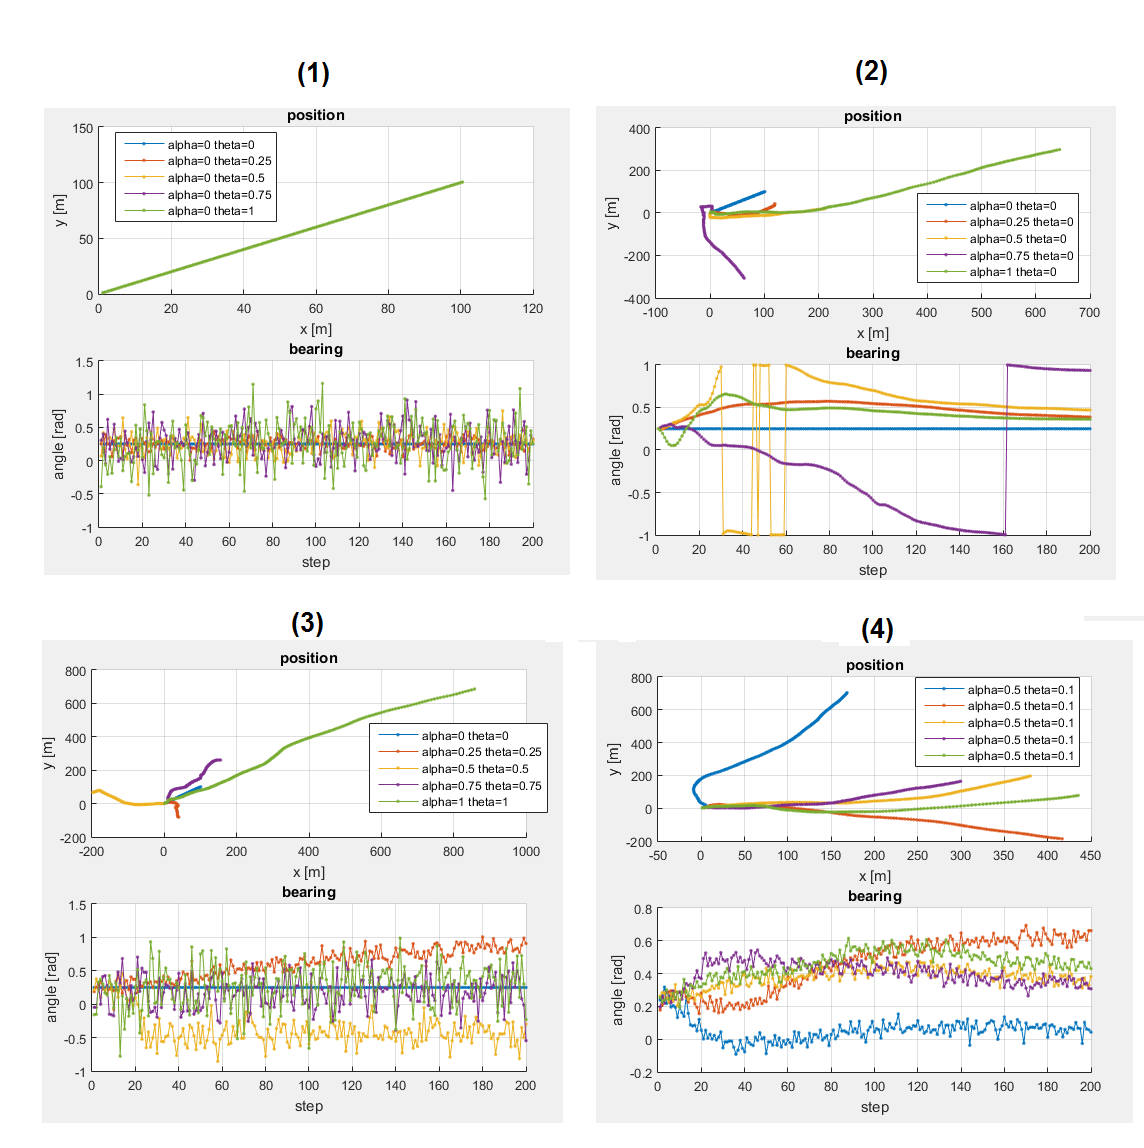
\includegraphics[width=\textwidth,height=\textheight,keepaspectratio]{q2.png}
\end{figure}




%%%%%%%%%%%%%%%%%%%%%%%%%%%%%%%%%%%%%%%%%%%%%%%%%%%%%%%%%%%
%%%%%%%%%%%%%%%%%%%%%%%%%%%%%%%%%%%%%%%%%%%%%%%%%%%%%%%%%%%

\section*{Question 3}
\begin{figure}
   \caption{\label{q3a} }
   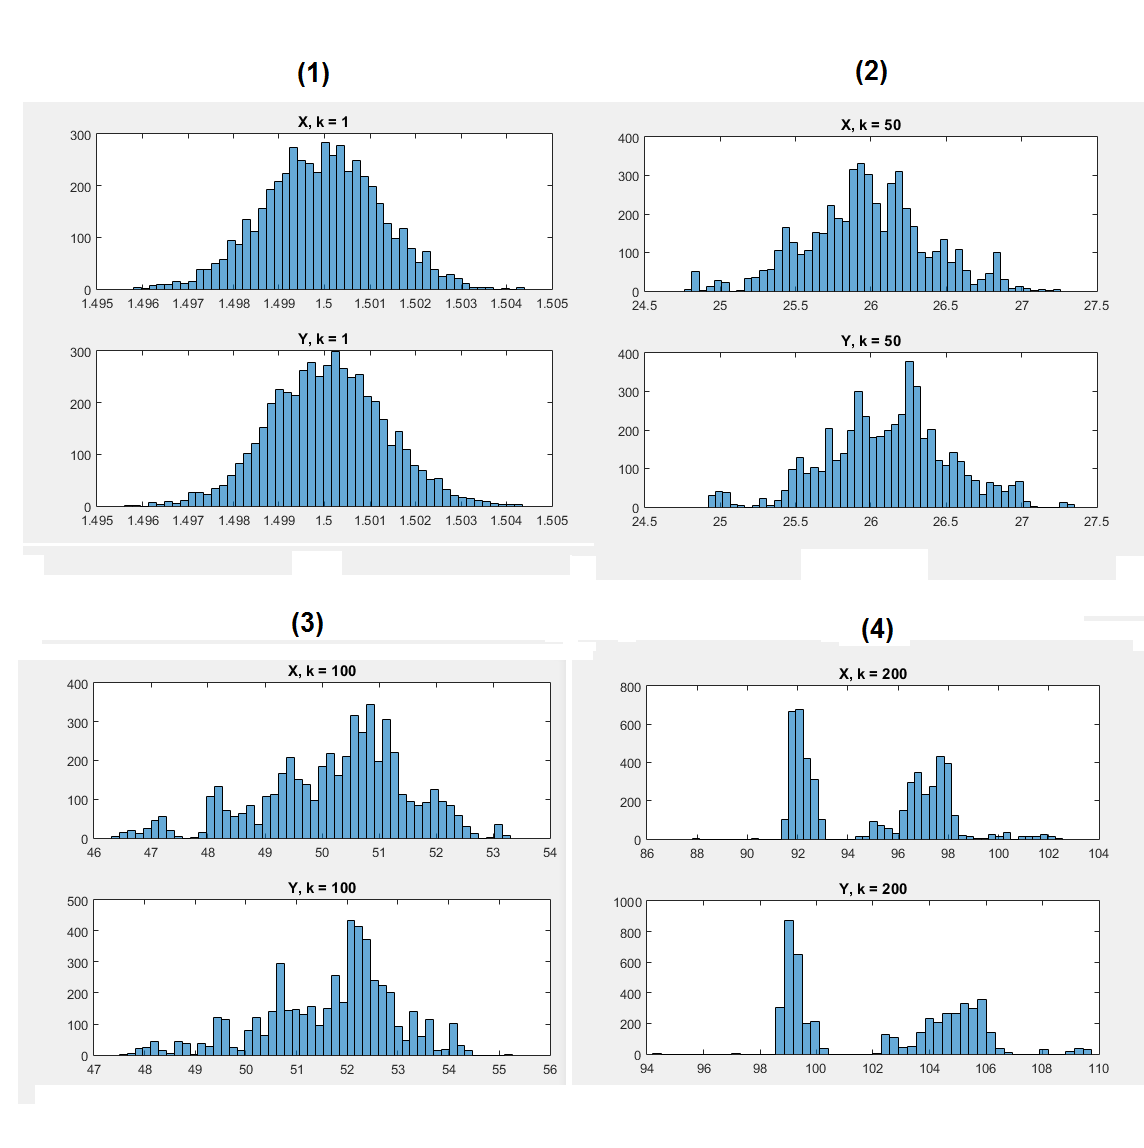
\includegraphics[width=\textwidth,height=\textheight,keepaspectratio]{q3a.png}
\end{figure}
\begin{figure}
\begin{center}
   \caption{\label{q3b} }
   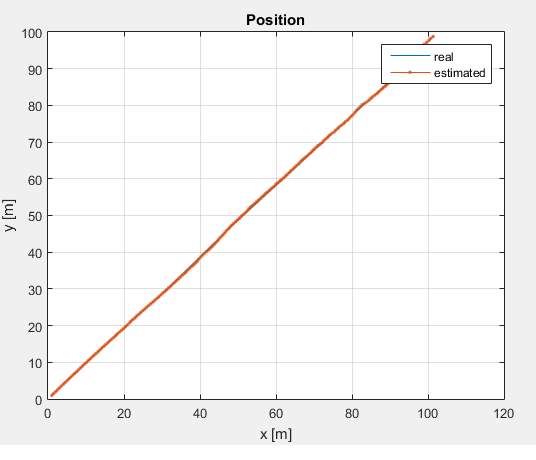
\includegraphics[width=10cm,height=\textheight,keepaspectratio]{q3b.png}
\end{center}
\end{figure}



%%%%%%%%%%%%%%%%%%%%%%%%%%%%%%%%%%%%%%%%%%%%%%%%%%%%%%%%%%%
%%%%%%%%%%%%%%%%%%%%%%%%%%%%%%%%%%%%%%%%%%%%%%%%%%%%%%%%%%%

\section*{Question 4}
\begin{figure}
   \caption{\label{q4} }
   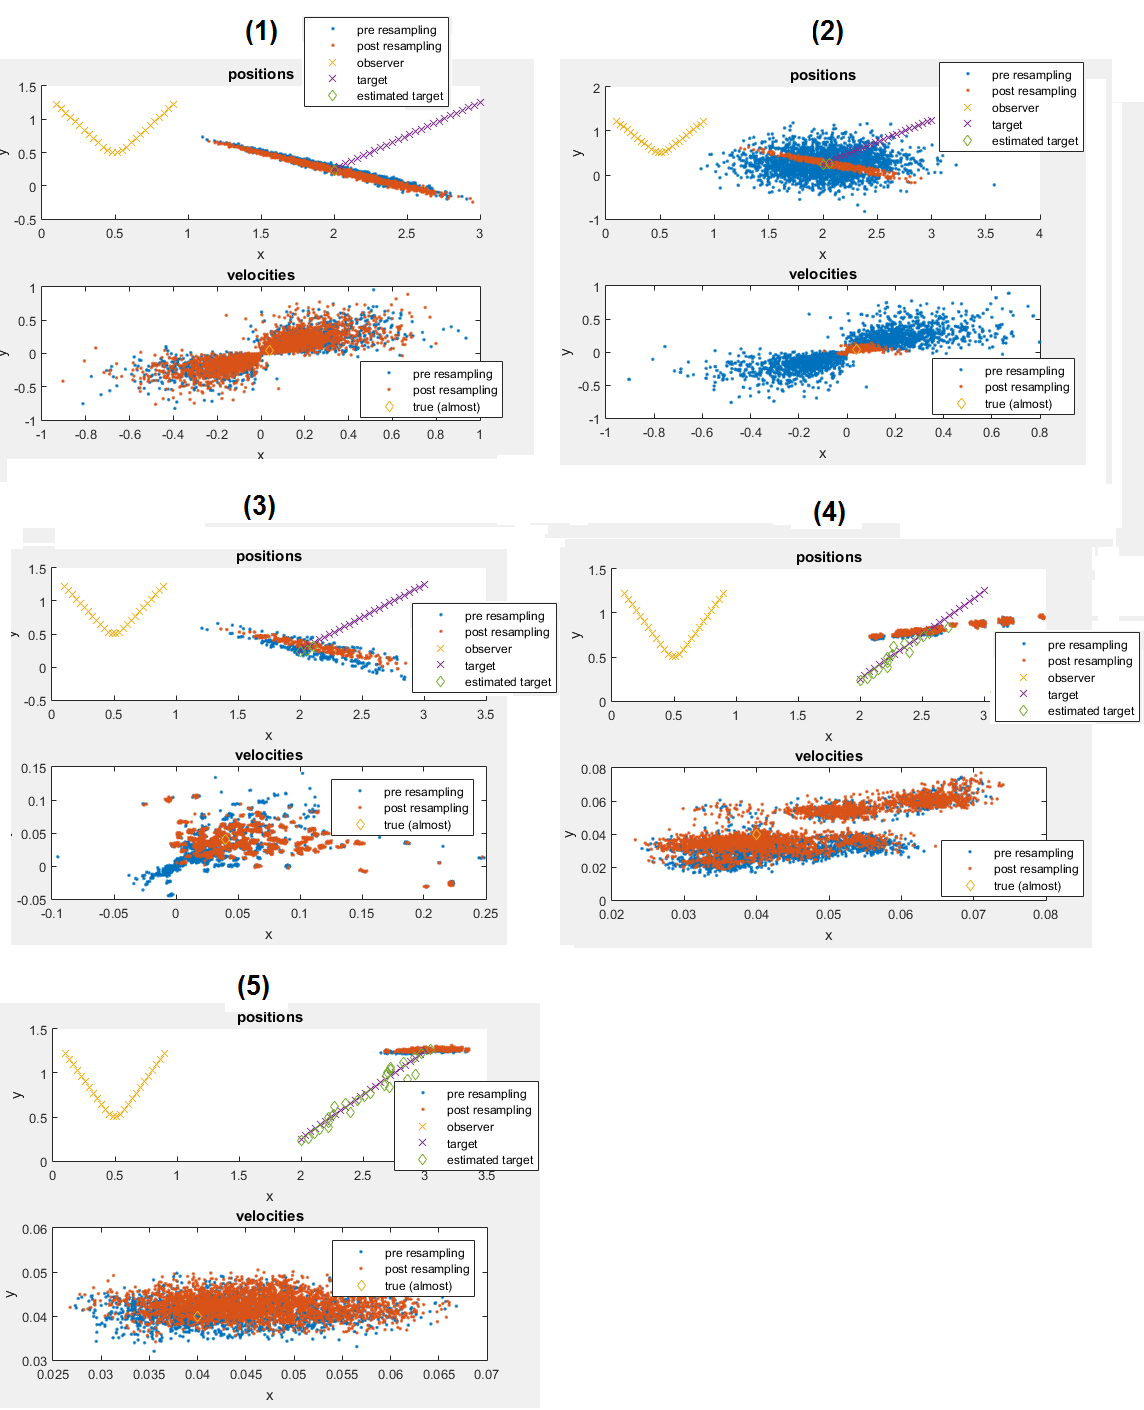
\includegraphics[width=\textwidth,height=\textheight,keepaspectratio]{q4.png}
\end{figure}




%%%%%%%%%%%%%%%%%%%%%%%%%%%%%%%%%%%%%%%%%%%%%%%%%%%%%%%%%%%
%%%%%%%%%%%%%%%%%%%%%%%%%%%%%%%%%%%%%%%%%%%%%%%%%%%%%%%%%%%

\section*{Question 5}





%%%%%%%%%%%%%%%%%%%%%%%%%%%%%%%%%%%%%%%%%%%%%%%%%%%%%%%%%%%
%%%%%%%%%%%%%%%%%%%%%%%%%%%%%%%%%%%%%%%%%%%%%%%%%%%%%%%%%%%

\section*{Question 6}




\lstinputlisting{q2.m}


\end{document}